% Drawing 86/02-3 -- folder 86, batch 02, archive page 29 (PDF page 30).
% Transcription: sous un croquis de pentagone à diagonales, de sommets $u$, $v$, marqué $a$, $s$, $f$
% Kind: pentagon with diagonals (margin). Method 2 (schematic redraw from the facsimile). Status: partial.
% Notes: Pentagon with two diagonals, one thickened; labels u, s, f, a placed as read on the crop. The vertex v of the transcription is not identified with certainty and is left unlabelled; the marginal "NB a ~ {u, v}" under it is text and left out.
% Coordinates: 1 unit = 1 mm = 1/100 of the crop width (bbox in page fractions: [0.1, 0.42, 0.28, 0.52]).
% Redrawn by Claude (claude-opus-5-5), issue #73, 2026-11-07; not checked by a human; not compiled (no TeX in the session).
% Rights: reproduces part of the work -- behind RENDER_TRANSCRIPTS, never published by itself.
\documentclass[tikz,border=3pt]{standalone}
\usepackage{amsmath,amssymb}
\usetikzlibrary{patterns,arrows.meta}
\tikzset{pencil/.style={black!45}, struck/.style={black!35}, mark/.style={circle,draw,inner sep=1.3pt}, pt/.style={circle,fill,inner sep=0.9pt}, opt/.style={circle,draw,fill=white,inner sep=1.1pt}}
\begin{document}
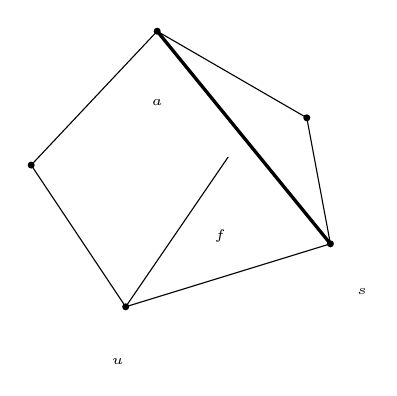
\begin{tikzpicture}[x=1mm,y=1mm,line cap=round,line join=round,font=\scriptsize]
\draw (38,-15) -- (57,-26) -- (60,-42) -- (34,-50) -- (22,-32) -- cycle;
\draw[very thick] (38,-15) -- (60,-42);
\draw (34,-50) -- (47,-31);
\node[pt] at (38,-15) {};
\node[pt] at (57,-26) {};
\node[pt] at (60,-42) {};
\node[pt] at (34,-50) {};
\node[pt] at (22,-32) {};
\node[inner sep=1pt] at (38,-24) {\tiny $a$};
\node[inner sep=1pt] at (46,-41) {\tiny $f$};
\node[inner sep=1pt] at (64,-48) {\tiny $s$};
\node[inner sep=1pt] at (33,-57) {\tiny $u$};
\end{tikzpicture}
\end{document}
